\documentclass[11pt]{article}
\usepackage{amsmath}
\usepackage{amssymb}
\usepackage[margin=.5in,left=.5in]{geometry} 
\usepackage{amsthm}
\usepackage{pgfplots}
\pgfplotsset{compat=1.18}
\setlength{\parindent}{0pt}

\begin{document}

\begin{titlepage}
    \centering
    \vspace*{\fill} % Push content to vertical center
    {\Large Ordinary Differential Equations} \\[0.5cm]
    {\Large Chapter 1.2 Notes: Solutions \& Inital Value Problems} \\[0.5cm]
    {\large Victor C. Van} \\[1cm]
    {\large December 19, 2024}
    \vspace*{\fill} % Push content to vertical center
\end{titlepage}

An \textit{n}th order ordinary differential equation is an equality involving the independent variable x,  the dependent variable y, and the first \textit{n} derivative of y.
Examples are:

\[
    \text{Second Order}: x^{2} + \frac{d^{2}y}{dx^{2}} + y = x^{3}
\]

\[
    \text{Second Order}: \sqrt{1- (\frac{d^{2}y}{dx^{2}})^{2}} - y = 0
\]

\[
    \text{Fourth Order}: \frac{d^{4}y}{dx^{4}} = xy
\]

Thus a general form for an nth order equation would be:

\[
    F(x,y, \frac{dy}{dx}, \cdots, \frac{d^{n}y}{dx^{n}} = 0) \tag{1}
\]

where \textit{F} is a function of the independent variable x, the dependent variable y, and the derivative of y up to order n; that is $x,y, \cdots, \frac{d^{n-1}y}{dx^{n-1}}$.
We assume thst the equation holds for all x in an interval \textit{I} (which masy or may not include its endpoints:
$a \leq x \leq b, a < x \leq b, etc).$ In many cases, we can isolate the highest-order term $\frac{d^{n}y}{dx^{n}}$, and write (1) as:

\[
    \frac{d^{n}y}{dx^{n}} = f(x,y, \frac{dy}{dx}, \cdots, \frac{d^{n}y}{dx^{n}}) \tag{2}
\]

which is often preferable to (1) for theoretical and computational purposes.


\fbox{
\begin{minipage}{0.95\linewidth} % Adjust the width as needed
\textbf{EXPLICIT SOLUTION}\\
\textbf{Definition 1.} A function $\phi(x)$ that when substituted for $y$ in equation (1) [or (2)] satisfies the equation for all $x$ in the interval \textit{I} is called an \textbf{explicit solution} to the equation on \textit{I}.
\end{minipage}}

\textbf{EXAMPLE 1:} Show that $\phi(x) = x^{2} - x^{-1}$ is an explicit solution today

\[
    \frac{d^{2}y}{dx^{2}} - \frac{2}{x^{2}}y = 0.
\]

\textbf{Solution}: The functions $\phi(x) = x^{2} - x^{-1}, \phi'(x) = 2x + x^{-2}$, and $\phi''(x) = 2 - 2x^{-3}$ are defined for all
$x \not = 0$. Substitution of $\phi(x)$ for $y$ in the equation (3) gives:

\[
    (2-2x^{-3})- \frac{2}{x^{2}}(x^{2}-x^{-1}) =  (2-2x^{-3}) - (2-2x^{-3}) = 0.
\]

\textbf{EXAMPLE 2:} Show that for \textit{any} choice of the constants $c_1$ and $c_2$, the function

\[
    \phi(x) = c_{1}e^{-1} + c_2e^{2x}
\]

is an explicit solution to

\[
    y'' -  y' -2y = 0. \tag{4}
\]

\textbf{Solution}: We compute $\phi'(x) = -c_1e^{-x} + 2c_2e^{2x} and \phi''(x) = c_1e^{-1}+4c_2e^{2x}.$
Substitution of $\phi$, $\phi'$, $\phi''$ for $y$, $y'$, and $y''$ in equation (4) yields:

\[
    (c_1e^{-1}+4c_2e^{2x}) - (-c_1e^{-x} + 2c_2e^{2x}) - 2(c_1e^{-x}+c_2e^{2x})
\]

\[
    = (c_1 + c_1 -2c_1)e^{-x} + (4c_2-2c_2-2c_2)e^{2x} = 0.
\]

Since equality holds for all x in $(- \infty, \infty)$, then $\phi(x) = c_1e^{-1} + c_2e^{2x}$ is an explicit solution to (4) on the interval $(- \infty, \infty)$ for any choice of the constants $c_1$ and $c_2$.

\newpage

\fbox{
\begin{minipage}{0.95\linewidth} % Adjust the width as needed
\textbf{IMPLICIT SOLUTION}\\
\textbf{Definition 2.} A relation $G(x,y) = 0$ is said to be an \textbf{implicit solution} to an equation (1) on the interval \textit{I} if it defines one or more explicit solutions on \textit{I}.
\end{minipage}}

\textbf{EXAMPLE 5:} Verify that $4x^{2}-y^{2}=C$, where $C$ is an arbitrary constant, gives a one-parameter family of implicit solutions to:
\[
    y \frac{dy}{dx} - 4x = 0 \tag{9},
\]

and graph several of these solution curves.

\textbf{Solution}: When we implicitly differentiate the equation $4x^{2} - y^{2} = C$ with respect to x, we find

\[
    8x - 2y \frac{dy}{dx} = 0,
\]

which is equivalent to (9). In figure 1.4 we have sketchedthe implicit solutions for $C = 0, \pm 1, \pm 4$.
The curves are hyperbolas with common asymptotes $ y = \pm 2x$. Notice that the implicit solution curves (with $C$ arbitrary)
fill the entire plane and are nonintersecting for $C \not = 0$. For $C=0$, the implicit solution gives rise to the two explicit solutions $y=2x$ and $y=-2x$, 
both of which passes through the origin.

\begin{center}
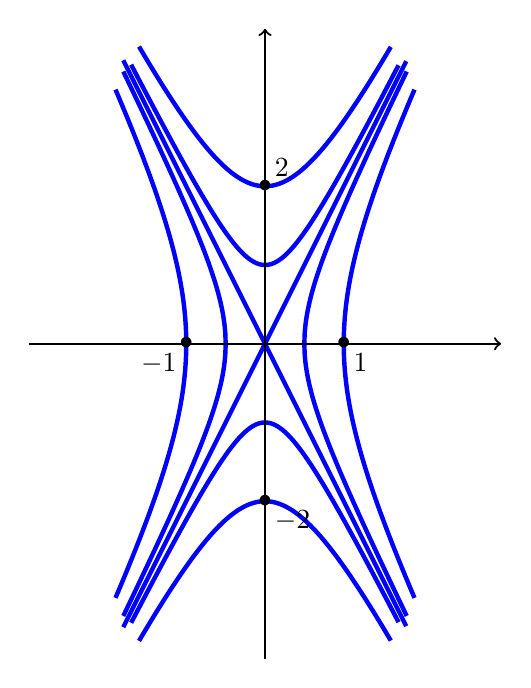
\begin{tikzpicture}
    % C=1 curves
    \draw[ultra thick,blue,domain=.5:1.8,samples=500] plot (\x,{sqrt(4*\x*\x-1)});
    \draw[ultra thick,blue,domain=.5:1.8,samples=500] plot (\x,{-sqrt(4*\x*\x-1)});
    \draw[ultra thick,blue,domain=.5:1.8,samples=500] plot (-\x,{sqrt(4*\x*\x-1)});
    \draw[ultra thick,blue,domain=.5:1.8,samples=500] plot (-\x,{-sqrt(4*\x*\x-1)});
    % C=4 curves
    \draw[ultra thick,blue,domain=1:1.9,samples=500] plot (\x,{sqrt(4*\x*\x-4)});
    \draw[ultra thick,blue,domain=1:1.9,samples=500] plot (\x,{-sqrt(4*\x*\x-4)});
    \draw[ultra thick,blue,domain=1:1.9,samples=500] plot (-\x,{sqrt(4*\x*\x-4)});
    \draw[ultra thick,blue,domain=1:1.9,samples=500] plot (-\x,{-sqrt(4*\x*\x-4)});
    % C=-1 curves
    \draw[ultra thick,blue,domain=-1.7:1.7,samples=500] plot (\x,{sqrt(4*\x*\x+1)});
    \draw[ultra thick,blue,domain=-1.7:1.7,samples=500] plot (\x,{-sqrt(4*\x*\x+1)});
    % C=-4 curves
    \draw[ultra thick,blue,domain=-1.6:1.6,samples=500] plot (\x,{sqrt(4*\x*\x+4)});
    \draw[ultra thick,blue,domain=-1.6:1.6,samples=500] plot (\x,{-sqrt(4*\x*\x+4)});
    % C=0 curves
    \draw[ultra thick,blue,domain=-1.8:1.8,samples=500] plot (\x,{sqrt(4*\x*\x)});
    \draw[ultra thick,blue,domain=-1.8:1.8,samples=500] plot (\x,{-sqrt(4*\x*\x)});
    % the grid and the points
    \draw[thick,->] (-3,0)--(3,0);
    \draw[thick,->] (0,-4)--(0,4);
    \draw (1,0) node {$\bullet$} node[below right] {$1$};
    \draw (-1,0) node {$\bullet$} node[below left] {$-1$};
    \draw (0,2) node {$\bullet$} node[above right] {$2$};
    \draw (0,-2) node {$\bullet$} node[below right] {$-2$};
\end{tikzpicture}
\end{center}

\begin{center}
    \[
        \tag{Figure 1.4 Implicit solutions $4x^{2}-y^{2}=C$} 
    \]
\end{center}

\newpage

\fbox{
\begin{minipage}{0.95\linewidth} % Adjust the width as needed
\textbf{INITIAL VALUE PROBLEM}\\

\textbf{Definition 3.} 

By an \textbf{initial value problem} for an \textit{n} th order differential equation
\[
    F(x,y, \frac{dy}{dx}, \cdots, \frac{d^{n}y}{dx^{n}}) = 0,
\]
we mean: Find a solution to the differential equation on an interval \textit{I} that satisfies at $x_0$ the \textit{n} initial conditions

\[
    y(x_0) = 0;
\]

\[
    \frac{dy}{dx} (x_0) = y
\]


\[
    \frac{d^{n-1}y}{dx^{n-1}} (x_0) = y_{n-1}
\]

\end{minipage}}

\fbox{
\begin{minipage}{0.95\linewidth} % Adjust the width as needed
\textbf{EXISTENCE \& UNIQUENESS OF SOLUTION}\\

\textbf{Theorem 1.} 
Given the initial value problem
\[
    \frac{dy}{dx} = f(x,y), y(x_0) = y_0,
\]  
assume that $f$ and $\frac{ \partial f}{ \partial y}$ are continious functions in a rectange

\[
R = \{(x,y) \mid a < x < b, c < y < d \}
\]

that contains the point $(x_0,y_0)$. Then the initial value problem has a unique solution $\phi(x)$
in some interval $x_0-h < x < x_0 + h$, where h is a positive number.

\end{minipage}}

\end{document}